  Afin de détecter les carrés du \rubic{}, nous avons étudié la variance entre les points voisins de l'image. 
En faisant l'hypothèse que les carrés du cube sont là où la variance varie le moins dans l'image. 

\subsubsection*{Principe de la méthode} 

  Contrairement aux images précédentes, nous travaillons directement avec l'image sans utiliser les projections en X et en Y. 

Cette méthode peut se décomposer en plusieurs étapes : 
\begin{enumerate}
  \item Calcul de la variance de l'image : \\
  Nous déterminons un entier qui correpond à la taille (hauteur et largeur) de la fenêtre qui va parcourir l'image. 
La variance est calculée sur chacune de ces fenêtres pour obtenir une matrice contenant les variances sur toutes ces fenêtres. 

On obtient une matrice qui est représentée comme dans la figure~\ref{variance2D_VARavant}. 

\begin{figure}[!ht]
\centering
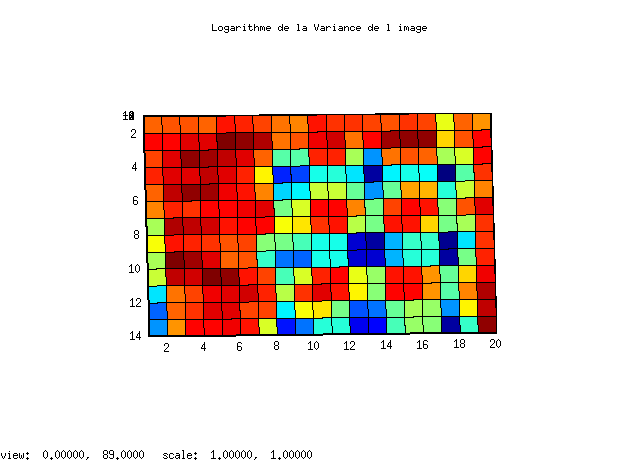
\includegraphics[width=\linewidth]{Images/Variance2D_variance_avan_2.png}
\caption{Variance obtenue pour l'image conf4/face4}
\label{variance2D_VARavant}
\end{figure}

  Pour rappel, le bleu correspond aux valeurs de variance les plus faibles alors que le rouge correspond aux valeurs élevées.
On voit apparaître les faces du \rubic{}. 

  On remarque cependant qu'il y a en bas à gauche, un zone bleue qui peut poser problème lors de la détection des plats. 

  \item Recherche des plats : \\
 
  Pour rechercher les plats, on a pris les minimums de variance successifs de la matrice de Variance sachant que pour chaque minimum détécté, nous avons changé sa valeur et celle de ces voisins afin que ce plat ne soit pas détécté à l'itération suivante. 

  Un plat est donc représenté par un point ayant des coordonnées X et Y et qui correspond à l'estimation du centre du carré du \rubic.

 La matrice modifiée devient la figure~\ref{variance2D_VARapres}. 

\begin{figure}[!ht]
\centering
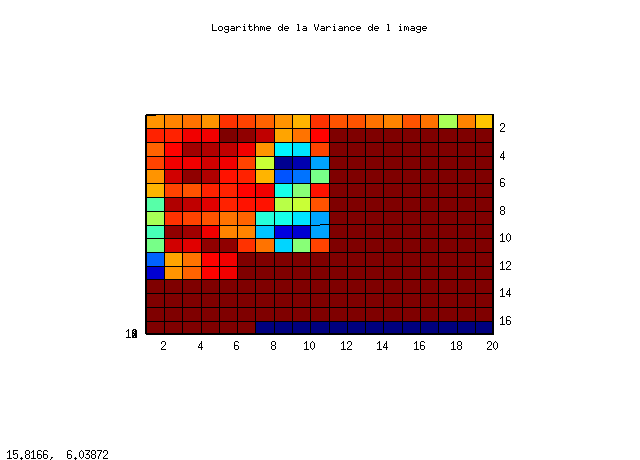
\includegraphics[width=\linewidth]{Images/Variance2D_variance_apres_2.png}
\caption{Variance obtenue pour l'image conf4/face4}
\label{variance2D_VARapres}
\end{figure}

  Nous pouvons constater que la zone qui posait problème précédemment a bien été séléctionnée comme un plat. 
Il faut donc faire un tri qui permettrait de détecter ce genre d'erreur. 

  \item Tri des plats : \\ 

  Pour trier les plats, nous avons utilisé la matrice de distance entre les plats. 
Nous avons fait notre choix de garder ou supprimer un plat en fonction de sa distance mimimale avec les autres plats. 
Ainsi tous les plats dont cette distance est inférieure à un seuil sont supprimés. 
Plus ce seuil est faible, plus il nous réduit le critère d'alignement des points. 

  Ce critère est appliqué pour chaque plat sur leurs absisses et leurs ordonnées. 

  \item Interpolation des plats manquants : \\

  Nous avons maintenant un nombre de plat inférieur à celui dont nous avons besoin pour retrouver les 9 carrés du \rubic{}. 

  Nous avons pour résoudre ce problème diviser l'image du cube en plusieurs zones qui correspondent aux emplacements les plus succeptibles de contenir une face. 
  Ce découpage en zone est défini comme présenté dans la figure ~\ref{variance2D_zone}. 

\begin{figure}[!ht]
\centering
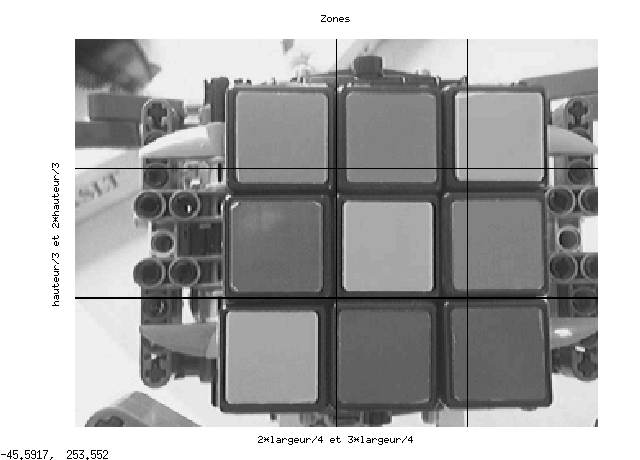
\includegraphics[width=\linewidth]{Images/Variance2D_zone.png} 
\caption{Zone de probabilité d'apparition d'une face} 
\label{variance2D_zone}
\end{figure}

  Pour ajouter des points nous avons récupérer grâce à la fonction \textit{unique} les coordonnées X et Y des plats validés. 
Nous avons noté lX et lY le nombre d'absisse et le nombre d'ordonnée appartenant à des plats validés et nous avons traité les cas suivants : lX égale 1, 2, 3 ou 4 et lY égale 1, 2, 3 ou 4. 
De plus, on note dX et dY la distance minimale entre les plats restants qui est l'approximation de la distance entre deux plats voisins. 

Les cas pour lX ont été traités de la façon suivante : 
  \begin{itemize}
    \item $lX=1$ : En fonction de la zone où est le plat valide, on ajoute deux plats de même absisse dans les zones libres tel qu'il y ait une distance dY entre ces points . 
    \item $lX=2$ : En fonction de la zone où sont les plats valides, on ajoute un dernier plat de même absisse dans la zone libre tel qu'il y ait une distance dX entre ces points . 
    \item $lX=3$ : On garde ces trois plats valides. 
    \item $lX=4$ : On a décidé de supprimer un plat dont la distance minimale avec les autres plats est la plus grande. 
  \end{itemize}

  Cependant si lX et lY valent 1 ou si une de ces deux variables est suppérieure à 4, la fonction renvoie une erreur. 
De même, si un plat est ajouté alors que ces coordonnées approximés sortent de l'image, une erreur est retournée. 
\end{enumerate}

  La signature de la fonctions créée est la suivantes : \\
\textit{function [plat, erreur] = detectionPlatVariance2D\_coord(image, largeurFenetre)}


\subsubsection*{Résultats obtenus par cette méthode}

  Les figures~\ref{variance2D_resultat_1} et ~\ref{variance2D_resultat_2} présentent les résultats obtenus pour deux images avec la méthode de la variance 2D : 

\begin{figure}[!ht]
\centering
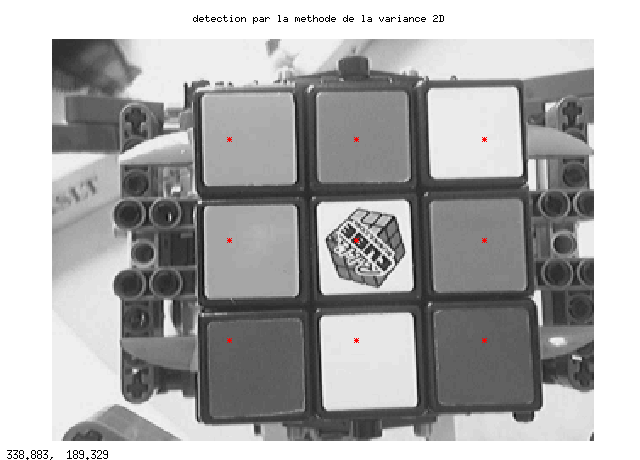
\includegraphics[width=0.6\linewidth]{Images/Variance2D_img_apres_1.png} 
\caption{Résultat de la méthode variance 2D} 
\label{variance2D_resultat_1}
\end{figure}

\begin{figure}[!ht]
\centering
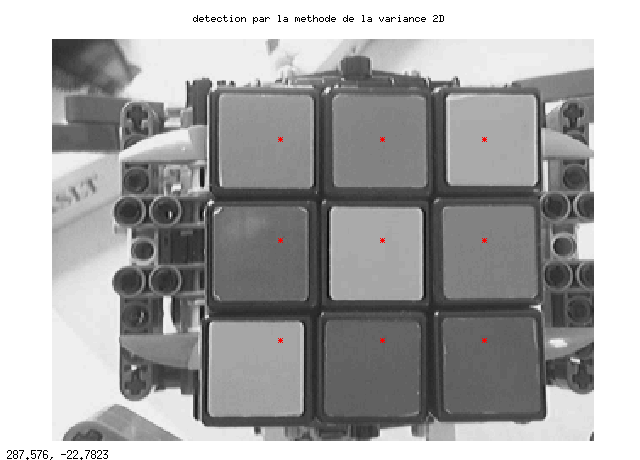
\includegraphics[width=0.6\linewidth]{Images/Variance2D_img_apres_2.png}
\caption{Résultat de la méthode variance 2D} 
\label{variance2D_resultat_2}
\end{figure}

  On remarque que les résultats sont exacts lorsque l'on est dans le cas de la face blanche ``spéciale'',de la face orientée et de celle non-orientée. 
  Cependant la face ayant des reflets obtient de mauvais résultats. 
